\documentclass{article}\usepackage[]{graphicx}\usepackage[]{color}
% maxwidth is the original width if it is less than linewidth
% otherwise use linewidth (to make sure the graphics do not exceed the margin)
\makeatletter
\def\maxwidth{ %
  \ifdim\Gin@nat@width>\linewidth
    \linewidth
  \else
    \Gin@nat@width
  \fi
}
\makeatother

\definecolor{fgcolor}{rgb}{0.345, 0.345, 0.345}
\makeatletter
\@ifundefined{AddToHook}{}{\AddToHook{package/xcolor/after}{\definecolor{fgcolor}{rgb}{0.345, 0.345, 0.345}}}
\makeatother
\newcommand{\hlnum}[1]{\textcolor[rgb]{0.686,0.059,0.569}{#1}}%
\newcommand{\hlstr}[1]{\textcolor[rgb]{0.192,0.494,0.8}{#1}}%
\newcommand{\hlcom}[1]{\textcolor[rgb]{0.678,0.584,0.686}{\textit{#1}}}%
\newcommand{\hlopt}[1]{\textcolor[rgb]{0,0,0}{#1}}%
\newcommand{\hlstd}[1]{\textcolor[rgb]{0.345,0.345,0.345}{#1}}%
\newcommand{\hlkwa}[1]{\textcolor[rgb]{0.161,0.373,0.58}{\textbf{#1}}}%
\newcommand{\hlkwb}[1]{\textcolor[rgb]{0.69,0.353,0.396}{#1}}%
\newcommand{\hlkwc}[1]{\textcolor[rgb]{0.333,0.667,0.333}{#1}}%
\newcommand{\hlkwd}[1]{\textcolor[rgb]{0.737,0.353,0.396}{\textbf{#1}}}%
\let\hlipl\hlkwb

\usepackage{framed}
\makeatletter
\newenvironment{kframe}{%
 \def\at@end@of@kframe{}%
 \ifinner\ifhmode%
  \def\at@end@of@kframe{\end{minipage}}%
  \begin{minipage}{\columnwidth}%
 \fi\fi%
 \def\FrameCommand##1{\hskip\@totalleftmargin \hskip-\fboxsep
 \colorbox{shadecolor}{##1}\hskip-\fboxsep
     % There is no \\@totalrightmargin, so:
     \hskip-\linewidth \hskip-\@totalleftmargin \hskip\columnwidth}%
 \MakeFramed {\advance\hsize-\width
   \@totalleftmargin\z@ \linewidth\hsize
   \@setminipage}}%
 {\par\unskip\endMakeFramed%
 \at@end@of@kframe}
\makeatother

\definecolor{shadecolor}{rgb}{.97, .97, .97}
\definecolor{messagecolor}{rgb}{0, 0, 0}
\definecolor{warningcolor}{rgb}{1, 0, 1}
\definecolor{errorcolor}{rgb}{1, 0, 0}
\makeatletter
\@ifundefined{AddToHook}{}{\AddToHook{package/xcolor/after}{
\definecolor{shadecolor}{rgb}{.97, .97, .97}
\definecolor{messagecolor}{rgb}{0, 0, 0}
\definecolor{warningcolor}{rgb}{1, 0, 1}
\definecolor{errorcolor}{rgb}{1, 0, 0}
}}
\makeatother
\newenvironment{knitrout}{}{} % an empty environment to be redefined in TeX

\usepackage{alltt}
\usepackage{hyperref}
%\usepackage{expl3}
%\usepackage{l3regex}
%\usepackage[version=4]{mhchem}
% \usepackage{animate}













\title{Weather Station Records and Communicating Climate Change--Mississippi}
%\subtitle{test}
\author{Marc Los Huertos}
\IfFileExists{upquote.sty}{\usepackage{upquote}}{}
\begin{document}

\maketitle

\tableofcontents

\section{Evaluating Terrestrial Meteorological Data}

\subsection{Selected History of Climate Science}

Geologists have known the climate has been changing over the Earth's history. But what causes these changes has been a major research area for over 100 years. There are numerous drivers that contribute to changing climates -- including the arrangement of the continents on the planet, the distance to the sun, energy generated by the sun, volanic activity, and the composition of the Earth's atmosphere. 

It's the last one that we'll spend time because the Earth's temperature are changing pretty dramatically over the last 100 years and the cause is no mystery -- the human activity that has released carbon dioxide (CO$_2$) into the atmosphere. The two main sources of CO$_2$ is from land use change, e.g. deforestration, and the burning of fossil fuels, e.g. coal, oil, and natural gas. 

The first to propose the role of CO$_2$ on the Earth's atmosphere was a Swedish scientist Svante Arrhenius, who figured out that CO$_2$ absorbs infarred light. Moreover, he deduced that the Earth's temperature was actually warmer than it might otherwise be if CO$_2$ was not part of the Earth's atmoshere. 

\subsection{Why Look at Individual Stations?}

I don't think there is a single, perfect way to analyze and communicate climate change. But the beauty of the network of stations in the USA and around the world is that these stations record weather as expecienced by local people. And while indiviudual stations may not represent the overall regional and global patterns well, this give us a mechanism to connect local experiences to regional or global processes. 

Of course, some may fixate on the local pattern and remain unconvinced of the larger context and for those folks, there may be better ways to communicated climate data. 

However, I would be remiss in failing to mention that some may fixate on local patterns and use these patterns to ignore or to dimiss the patterns in other regions. 

Finally, the impacts of climate change are highly specific to the region in question. Thus, once someone understands the impacts on climate change in their region, they my not be able to appreciate how differnet the climate impacts might affect other peoples, who maybe more vulneratble, around the globe. 

Thus, with these weaknessed in mind, I will pursue this project with an eye to address these other issues at later stages.

\subsection{Approach}

\subsubsection{NOAA Data Records}

The US National Oceanic and Atmospheric Adminstration (NOAA) maintains several sources of digital weather data from the USA and beyond. These data have been collected from stations around the country to support a wide range of human activities that include farming, aviation, shipping, and even armed conflict. 

At various times, these records have been used to evaluate long-term climate change with varying success. Without a doubt, these data are not perfect, but they remain that foundation of an effective adn professionally maintained environmental monitoring program that engenders integrity, even when facing budget cuts. 

I will use these data to select for a station with a long record for each state in the USA. Future projects might evaluate the record for stations around the world, but we will see about that. 

%ftp://ftp.ncdc.noaa.gov/pub/data/ghcn/v3/

\subsubsection{rNOAA Package and R}

R is an open source programming environment that has become one of the most popular tools for statiticians and data scientists. Capitalizing on the open source framework, a wide range of libraries or packages have been developed to faciliate data processing, analysis, and graphical displays. On such package is rNOAA developed to collect and display climate records stored on NOAA servers.

Using the package requires the use of a key. To maintain the integrity of the key, it's best to avoid posting the key in a public repository and to encryp the key to ensure it's not abused. 

\subsection{Selecting Weather Records by State}

There are numerous ways to analyze temperature records, where stations can be analyzed individually or records could be sampled and analyzed in spatially in grids. Each of these are valid approaches depending on the question to be addressed. 

In this case the question is ``Based on the longest state meterological record, is there a temperature trend?"

\subsubsection{Identify List of State IDs (FIPS)}

Using the rNOAA library in R, we can queary NOAA's database to identify station codes (FIPS) by state. With the states and some territories, there are 55 FIPS for US weather stations. 

rNOAA has a simple function to list for each of the states and the weather stations in each. I use ncdc\_locs() functions to select each state and ncdc\_station() to obtain the station ids with the longest records. 



The function queries the NOAA website and retrieves state codes, ``FIPS:XX''. Each state has a number of weather stations,\footnote{Project Idea: It would be nice to make a map of how concentrated the stations spatially.} some with a long record, some with a short record, and some with numerous interruptions. Our goal is to select a long record with few missing data. 

\subsubsection{Selection Stations}

With the state ids, we can evaluate the metadata for all the weather stations, which will work to get the longest records, using \texttt{ncdc\_stations()}. 

First, we subset the data for stations that actively collecting data. Then we'll sort to the active stations to find the one with the longest records. We will use these stations for our analysis. 

There were some records that didn't have robust TMAX/TMIN records, so there are some states that I had to manually select an alternative stations. 

\begin{knitrout}
\definecolor{shadecolor}{rgb}{0.969, 0.969, 0.969}\color{fgcolor}\begin{kframe}
\begin{alltt}
\hlstd{GSOM_Stations} \hlkwb{<-} \hlkwd{ncdc_stations}\hlstd{(}\hlkwc{datasetid}\hlstd{=}\hlstr{'GSOM'}\hlstd{,}
               \hlkwc{datatypeid} \hlstd{=} \hlkwd{c}\hlstd{(}\hlstr{"TMAX"}\hlstd{,} \hlstr{"TMIN"}\hlstd{),}
               \hlkwc{locationid}\hlstd{=fips}\hlopt{$}\hlstd{id,} \hlkwc{limit}\hlstd{=}\hlnum{1000}\hlstd{,}
               \hlkwc{sortfield} \hlstd{=} \hlstr{'maxdate'}\hlstd{,} \hlkwc{sortorder}\hlstd{=}\hlstr{'desc'}\hlstd{)}

\hlstd{GSOM_Recent} \hlkwb{=}
   \hlstd{GSOM_Stations}\hlopt{$}\hlstd{data[GSOM_Stations}\hlopt{$}\hlstd{data}\hlopt{$}\hlstd{maxdate}\hlopt{>=}\hlstr{'2021-11-01'}\hlstd{,]}

\hlstd{GSOM_Coverage} \hlkwb{=}
   \hlstd{GSOM_Recent[GSOM_Recent}\hlopt{$}\hlstd{datacoverage} \hlopt{>} \hlnum{0.92}\hlstd{,]}
\hlstd{GSOM_Sorted} \hlkwb{=}  \hlstd{GSOM_Coverage[}\hlkwd{order}\hlstd{(GSOM_Coverage}\hlopt{$}\hlstd{mindate),]}

\hlstd{GSOM_Longest} \hlkwb{=} \hlstd{GSOM_Sorted[}\hlnum{1}\hlstd{,]} \hlcom{#Pick longest}
\hlcom{# Second and Third for Comparisons}
\hlcom{# GSOM_Longest = GSOM_Sorted[2,] }
\hlcom{# GSOM_Longest = GSOM_Sorted[3,]}

\hlcom{# Exceptions Overrride by changing GSOM_Sorted[#,]}
\hlcom{# Iowa (same as Hawaii)}
\hlkwa{if}\hlstd{(fips}\hlopt{$}\hlstd{State}\hlopt{==}\hlstr{"Hawaii"}\hlstd{)\{}
   \hlkwd{print}\hlstd{(}\hlstr{"Manual Override for Hawaii"}\hlstd{)}
   \hlstd{GSOM_Longest} \hlkwb{=} \hlstd{GSOM_Sorted[}\hlnum{1}\hlstd{,]}
\hlstd{\}}


\hlcom{# Iowa (same as Illonois)}
\hlkwa{if}\hlstd{(fips}\hlopt{$}\hlstd{State}\hlopt{==}\hlstr{"Iowa"} \hlopt{|} \hlstd{fips}\hlopt{$}\hlstd{State}\hlopt{==}\hlstr{"Illinois"}\hlstd{)\{}
   \hlkwd{print}\hlstd{(}\hlstr{"Manual Override for Iowa/Illinois"}\hlstd{)}
   \hlstd{GSOM_Longest} \hlkwb{=} \hlstd{GSOM_Sorted[}\hlnum{2}\hlstd{,]}
\hlstd{\}}

\hlcom{# Pennsylvania}
\hlkwa{if}\hlstd{(fips}\hlopt{$}\hlstd{State}\hlopt{==}\hlstr{"Pennsylvania"}\hlstd{)\{}
   \hlkwd{print}\hlstd{(}\hlstr{"Manual Override for Penn"}\hlstd{)}
   \hlstd{GSOM_Longest} \hlkwb{=} \hlstd{GSOM_Sorted[}\hlnum{2}\hlstd{,]}
\hlstd{\}}

\hlcom{# South Dakota}

\hlcom{# Tennessee }
\hlkwa{if}\hlstd{(fips}\hlopt{$}\hlstd{State}\hlopt{==}\hlstr{"Tennessee"}\hlstd{)\{}
   \hlkwd{print}\hlstd{(}\hlstr{"Manual Override for Tennessee"}\hlstd{)}
   \hlstd{GSOM_Longest} \hlkwb{=} \hlstd{GSOM_Sorted[}\hlnum{2}\hlstd{,]}
\hlstd{\}}


\hlcom{#Puerto Rico}
\hlcom{# Puerto Rico}
\hlstd{PR} \hlkwb{=} \hlnum{0}
\hlkwa{if}\hlstd{(PR} \hlopt{==} \hlnum{1}\hlstd{)\{}
\hlstd{fips}\hlopt{$}\hlstd{State} \hlkwb{=} \hlstr{"Puerto Rico"}
\hlstd{fips}\hlopt{$}\hlstd{id} \hlkwb{=} \hlstr{"FIPS:PR"}

\hlstd{GSOM_Selected} \hlkwb{=} \hlkwd{ncdc_stations}\hlstd{(}\hlkwc{datasetid}\hlstd{=}\hlstr{"GSOM"}\hlstd{,}
                             \hlkwc{stationid} \hlstd{=} \hlstr{"GHCND:RQC00665097"}\hlstd{,}
                             \hlkwc{datatypeid} \hlstd{=} \hlkwd{c}\hlstd{(}\hlstr{"TMAX"}\hlstd{,} \hlstr{"TMIN"}\hlstd{))}
\hlstr{"Doing Puerto Rico"}
\hlstd{GSOM_Longest} \hlkwb{=} \hlstd{GSOM_Selected}\hlopt{$}\hlstd{data}

\hlstd{\}}

\hlstd{GQ} \hlkwb{=} \hlnum{0}
\hlkwa{if}\hlstd{(GQ}\hlopt{==} \hlnum{1}\hlstd{)\{}
\hlstd{fips}\hlopt{$}\hlstd{State} \hlkwb{=} \hlstr{"Guam"}
\hlstd{fips}\hlopt{$}\hlstd{id} \hlkwb{=} \hlstr{"FIPS:GQ"}

\hlstd{GSOM_Selected} \hlkwb{=} \hlkwd{ncdc_stations}\hlstd{(}\hlkwc{datasetid}\hlstd{=}\hlstr{"GSOM"}\hlstd{,}
                             \hlkwc{stationid} \hlstd{=} \hlstr{"GHCND:GQW00041415"}\hlstd{,}
                             \hlkwc{datatypeid} \hlstd{=} \hlkwd{c}\hlstd{(}\hlstr{"TMAX"}\hlstd{,} \hlstr{"TMIN"}\hlstd{))}

\hlstd{GSOM_Longest} \hlkwb{=} \hlstd{GSOM_Selected}\hlopt{$}\hlstd{data}
\hlstd{\}}

\hlkwd{str}\hlstd{(GSOM_Longest)}
\hlcom{# Change Case of Station Name -- Complicated!}
\hlcom{#v2 <- gsub("[sty]", "", paste(letters, collapse="")) }
\hlcom{#chartr(v2, toupper(v2), GSOM_Longest$name)}
\hlcom{#sub('\textbackslash{}\textbackslash{}b([a-z])([0-9])', '\textbackslash{}\textbackslash{}L\textbackslash{}\textbackslash{}1\textbackslash{}\textbackslash{}2', GSOM_Longest$name, perl=TRUE)}
\hlcom{#[1] "JAStADMMNIsyNDK" "LAUKsNDTUsAINS"}

\hlcom{# Caution this might be a problem!}
\hlstd{fips}\hlopt{$}\hlstd{State2} \hlkwb{<-} \hlkwd{sub}\hlstd{(}\hlstr{" "}\hlstd{,} \hlstr{"_"}\hlstd{, fips}\hlopt{$}\hlstd{State)}
\end{alltt}
\end{kframe}
\end{knitrout}

The record selected has the following metadata associated with it, which will be used for nameing, labeling, and mapping. 

   elevation    mindate    maxdate latitude            name datacoverage
45     143.3 1892-12-01 2022-04-01 34.24861 PONTOTOC, MS US       0.9569
                  id elevationUnit longitude
45 GHCND:USC00227106        METERS  -88.9975
[1] 1892
[1] 2022


\section{Gathering Weather Record Datasets}

\subsection{Main Datesets of Interest}

\begin{description}
  \item[GSOM]
  \item[CHCND]
  \item[CHCNM]
\end{description}

\subsection{Functions to Collect and Clean GSOM}

To collect the data, I used a short function, but the download time is painfully slow because only 1 year can be obtained at a time. Might want to get a work around for this at some point. 



Functions to bin data into decades and scores. 



The function relies on two inputs, the station id and the measured parameter -- TMAX and TMIN in this case. After that, the data needs to be clean up quite a bit. 

Furthermore, I have converted units to Farenheit, which is not my favorite, but important for US consumption.

\subsection{Functions to Report Probabilities}




\subsection{GSOM: Retreive and Clean Data}



\subsection{CHCND: Retreive and Clean Data}

CHCND have been bias corrected...


\section{Data Analysis Processes}

\subsection{Map Weather Station Location}

\begin{knitrout}
\definecolor{shadecolor}{rgb}{0.969, 0.969, 0.969}\color{fgcolor}\begin{kframe}


{\ttfamily\noindent\bfseries\color{errorcolor}{\#\# Error in eval(expr, envir, enclos): object 'AIzaSyDYUc3ExxqFTOHtyxyr6' not found}}\end{kframe}
\end{knitrout}




\begin{figure}
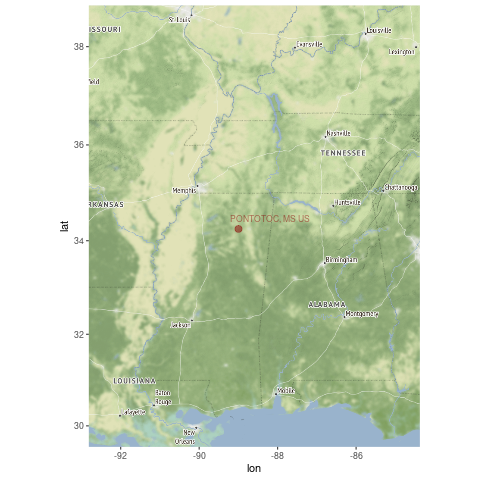
\includegraphics[width=1.00\textwidth]{/home/CAMPUS/mwl04747/github/Climate_Change_Narratives/Social_Media/State_htmls/png/Mississippi_USC00227106_MAP.png}
\caption{Weather Station Location (USC00227106). }
\label{fig:Map}
\end{figure}

\subsection{Using a Linear Model Monthy Trends}

I used a linear model (\texttt{lm()}) to evaluate the long term trend for each each month to determine which, if any, have long-term trends. At somepoint, I'll have to the stats correcting for the autocorrelation using a autoregressive model.  



Evaluate both TMAX and TMIN in GSOM by Year using MonthEvalStats() function. 




\subsubsection{Trends in Tabular Formats}

Admittedly, determining the months with the biggest changes isn't a very good approach for hypothesize testing -- it's more like a fishing expedition, but as long as we understand the difference between an a priori hypothesis and an exploratory analysis, we should be okay if we make appropriate conclusions. 



For this section, we'll look to see what months had the greatest changes for both TMIN and TMAX. By looking at significant slopes in whatever direction, we might learn if warming is really the dominiant pattern. 

Table~\ref{tab:TMINtrends} summarizes the monthly trends for TMAX.

\begin{table}[ht]
\centering
\begin{tabular}{rrrrrl}
  \hline
 & Month & Slope100 & r2 & p\_value & Symbol \\ 
  \hline
1 & 1 & -0.0484 & 0.13 & 0.0343 & * \\ 
  4 & 2 & -0.0445 & 0.13 & 0.0362 & * \\ 
  7 & 3 & -0.0475 & 0.15 & 0.0212 & * \\ 
  10 & 4 & -0.0031 & 0.00 & 0.8237 &  \\ 
  13 & 5 & -0.0138 & 0.04 & 0.2329 &  \\ 
  16 & 6 & -0.0268 & 0.18 & 0.0104 & * \\ 
  19 & 7 & -0.0236 & 0.21 & 0.0078 & ** \\ 
  22 & 8 & -0.0286 & 0.25 & 0.0025 & ** \\ 
  25 & 9 & -0.0079 & 0.01 & 0.5531 &  \\ 
  28 & 10 & -0.0252 & 0.07 & 0.1418 &  \\ 
  31 & 11 & -0.0072 & 0.01 & 0.6185 &  \\ 
  34 & 12 & -0.0125 & 0.01 & 0.5207 &  \\ 
   \hline
\end{tabular}
\caption{TMIN Trends} 
\end{table}


Table~\ref{tab:TMAXtrends} summarizes the monthly trends for TMAX.

% latex table generated in R 3.6.0 by xtable 1.8-4 package
% Thu Jun 30 07:47:19 2022
\begin{table}[ht]
\centering
\begin{tabular}{rrrrrl}
  \hline
 & Month & Slope100 & r2 & p\_value & Symbol \\ 
  \hline
2 & 1 & -0.0429 & 0.09 & 0.0833 &  \\ 
  5 & 2 & -0.0152 & 0.01 & 0.4999 &  \\ 
  8 & 3 & -0.0281 & 0.04 & 0.2334 &  \\ 
  11 & 4 & 0.0261 & 0.13 & 0.0347 & * \\ 
  14 & 5 & 0.0010 & 0.00 & 0.9250 &  \\ 
  17 & 6 & -0.0136 & 0.03 & 0.3294 &  \\ 
  20 & 7 & -0.0167 & 0.06 & 0.1817 &  \\ 
  23 & 8 & -0.0229 & 0.09 & 0.0799 &  \\ 
  26 & 9 & -0.0154 & 0.03 & 0.2886 &  \\ 
  29 & 10 & -0.0374 & 0.18 & 0.0123 & * \\ 
  32 & 11 & 0.0044 & 0.00 & 0.7274 &  \\ 
  35 & 12 & -0.0059 & 0.00 & 0.7722 &  \\ 
   \hline
\end{tabular}
\caption{TMAX Trends} 
\end{table}


PPT changes are tricky to capture and I'll have to keep working on this (Table~\ref{tab:PPTtrends}).

% latex table generated in R 3.6.0 by xtable 1.8-4 package
% Thu Jun 30 07:47:19 2022
\begin{table}[ht]
\centering
\begin{tabular}{rrrrrl}
  \hline
 & Month & Slope100 & r2 & p\_value & Symbol \\ 
  \hline
3 & 1 & -0.2679 & 0.02 & 0.3603 &  \\ 
  6 & 2 & -0.1303 & 0.01 & 0.6855 &  \\ 
  9 & 3 & -0.2519 & 0.02 & 0.4491 &  \\ 
  12 & 4 & 0.3942 & 0.04 & 0.2459 &  \\ 
  15 & 5 & 0.3246 & 0.07 & 0.1351 &  \\ 
  18 & 6 & -0.2939 & 0.03 & 0.2937 &  \\ 
  21 & 7 & 0.1549 & 0.01 & 0.6430 &  \\ 
  24 & 8 & -0.2693 & 0.05 & 0.2179 &  \\ 
  27 & 9 & 0.2114 & 0.02 & 0.3846 &  \\ 
  30 & 10 & 0.5012 & 0.12 & 0.0425 & * \\ 
  33 & 11 & -0.2027 & 0.01 & 0.5949 &  \\ 
  36 & 12 & 0.5020 & 0.06 & 0.1602 &  \\ 
   \hline
\end{tabular}
\end{table}


\subsubsection{Defining TMAXmonth and TMINmonth}


The greatest changes for Station GHCND:USC00227106

\section{Communicating Long-term Weather Records}

\subsection{Complete Records vs. Post 1975 Trends}

Communicating climate change based on station records is tricky. The long-term record would on the surface to be the most robust, but several issues arise with a naive analytical approach -- my favorite!

\begin{knitrout}
\definecolor{shadecolor}{rgb}{0.969, 0.969, 0.969}\color{fgcolor}\begin{kframe}


{\ttfamily\noindent\color{warningcolor}{\#\# Warning in predict.lm(GSOM.lm, newdata = pred\_dates, interval = "{}confidence"{}): prediction from a rank-deficient fit may be misleading}}

{\ttfamily\noindent\color{warningcolor}{\#\# Warning in qt((1 - level)/2, df): NaNs produced}}

{\ttfamily\noindent\color{warningcolor}{\#\# Warning in anova.lm(lm): ANOVA F-tests on an essentially perfect fit are unreliable}}

{\ttfamily\noindent\bfseries\color{errorcolor}{\#\# Error in if (anova(lm)\$"{}Pr(>F)"{}[1] > 0.05) \{: missing value where TRUE/FALSE needed}}\end{kframe}
\end{knitrout}

The noise in the data may suggests that no trend is present (Figure~\ref{fig:GSOM-1975trend}). It's tricky because the seasonal variation dominates the source of varition. In other words the intra-annual variation exceeds the inter-annual variation, making signal detection very difficult. Is there a way to "filter" out the seasonal effect? Yes, let's see how that works next. 

\begin{figure}
\includegraphics[width=1.00\textwidth]{/home/CAMPUS/mwl04747/github/Climate_Change_Narratives/Social_Media/State_htmls/png/Mississippi_USC00227106_GSOM_1975.png}
\caption{The climate trends from full record and post 1975 data. These data have a high level of variability due to seasonality effects that have not been filtered out.}
\label{fig:GSOM-1975trend}
\end{figure}


\subsection{Filtering Seasonal Effect}

There are several ways to filter out seasonal effects. The easiest way is subtract the mean value for each date, but that's tricky because every four years there is an extra day in Februrary -- although there are ways to deal with this, a more straight forward way is to use mean monthly values to capture the seasonality for each month. With 12 months, this is a pretty good approach because there is pretty good resolution. 

\subsubsection{Method 1: Filtering by Monthly Mean} 



\begin{knitrout}
\definecolor{shadecolor}{rgb}{0.969, 0.969, 0.969}\color{fgcolor}\begin{kframe}


{\ttfamily\noindent\color{warningcolor}{\#\# Warning in predict.lm(GSOM.lm, newdata = pred\_dates, interval = "{}confidence"{}): prediction from a rank-deficient fit may be misleading}}

{\ttfamily\noindent\color{warningcolor}{\#\# Warning in qt((1 - level)/2, df): NaNs produced}}

{\ttfamily\noindent\color{warningcolor}{\#\# Warning in anova.lm(lm): ANOVA F-tests on an essentially perfect fit are unreliable}}

{\ttfamily\noindent\bfseries\color{errorcolor}{\#\# Error in if (anova(lm)\$"{}Pr(>F)"{}[1] > 0.05) \{: missing value where TRUE/FALSE needed}}

{\ttfamily\noindent\color{warningcolor}{\#\# Warning in anova.lm(lm): ANOVA F-tests on an essentially perfect fit are unreliable}}

{\ttfamily\noindent\bfseries\color{errorcolor}{\#\# Error in if (anova(lm)\$"{}Pr(>F)"{}[1] > 0.05) \{: missing value where TRUE/FALSE needed}}\end{kframe}
\end{knitrout}

And to see what we created, see Figure~\ref{fig:GSOM-anomaly}.

\begin{figure}
\includegraphics[width=1.00\textwidth]{/home/CAMPUS/mwl04747/github/Climate_Change_Narratives/Social_Media/State_htmls/png/Mississippi_USC00227106_GSOM_anomaly_1975.png}
\caption{The changing in monthly temperature data.}
\label{fig:GSOM-anomaly}
\end{figure}

\subsubsection{Method 2: Polynomial Filter}

Project to be followed up with.

\begin{knitrout}
\definecolor{shadecolor}{rgb}{0.969, 0.969, 0.969}\color{fgcolor}\begin{kframe}
\begin{alltt}
\hlcom{# fit polynomial: x^2*b1 + x*b2 + ... + bn}

\hlcom{# create time series object}
\hlcom{#X = [i%365 for i in range(0, len(series))]}
\hlcom{# y = series.values}

\hlcom{# degree = 4}
\hlcom{#coef = polyfit(X, y, degree)}
\hlcom{# print('Coefficients: %s' % coef)}
\hlcom{# create curve}
\end{alltt}
\end{kframe}
\end{knitrout}


\subsection{Extreme Events--Using Daily Records}

\subsubsection{Complicated Nature of Rainfall Patterns}

Rainfall trends are tough. Exteme events can occur in 24 hours or over long periods that might result in floods or droughts. Each region might have different patterns, so developing a consistent approach is tough.

We can look for trends in monthly averages, number of days without rain (important in tropics), and/or extreme events based on daily or hourly data. 

I don't know of a robust way to look at this for the entire globe. 



Rainfall totals by season might be a useful way to think about changes, because the rainfall is often seasonal, I wonder if we can see pattners by season. 

\begin{knitrout}
\definecolor{shadecolor}{rgb}{0.969, 0.969, 0.969}\color{fgcolor}\begin{kframe}


{\ttfamily\noindent\itshape\color{messagecolor}{\#\# `geom\_smooth()` using formula 'y \textasciitilde{} x'}}\end{kframe}
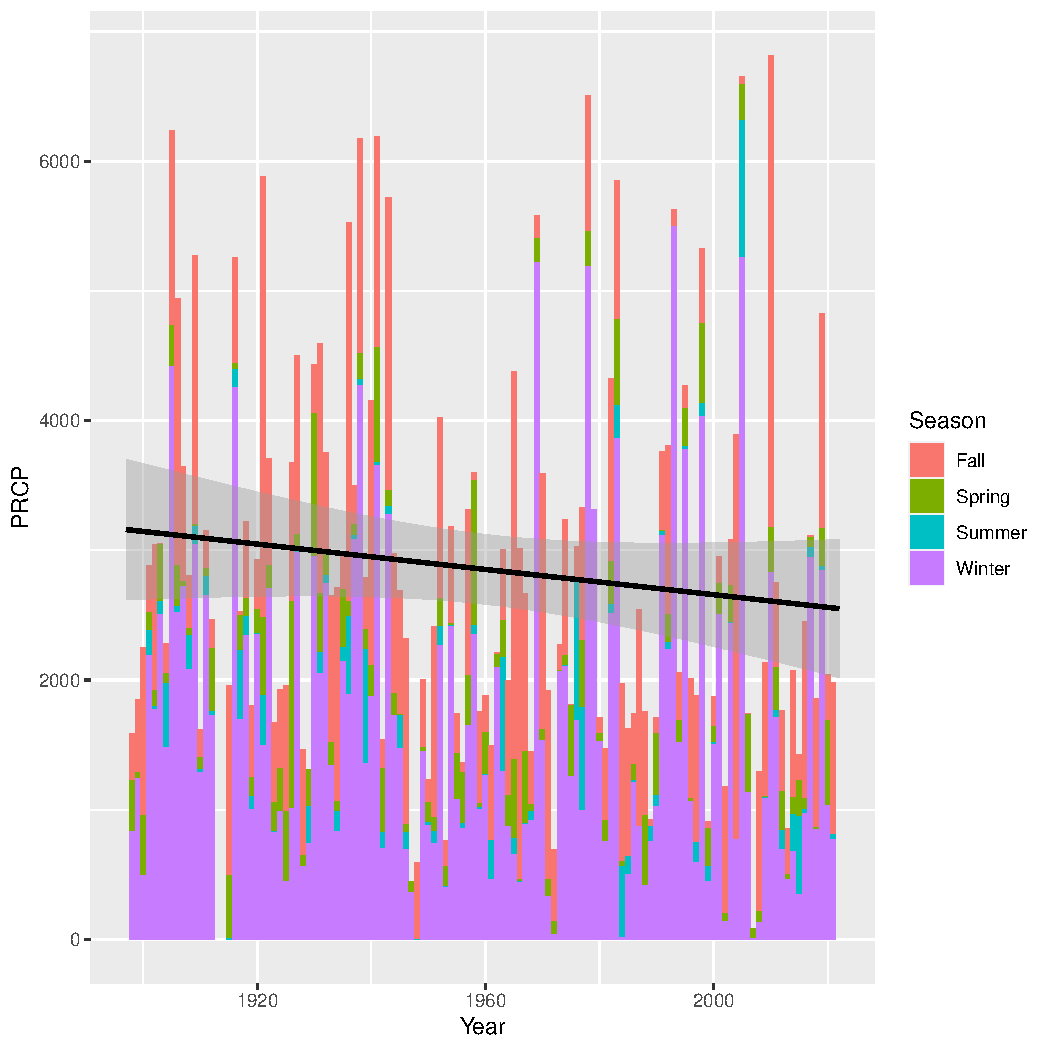
\includegraphics[width=\maxwidth]{figure/unnamed-chunk-9-1} 
\end{knitrout}

\subsubsection{Drought}

Days without rain...within a calendar year... bleed over between years isn't captured.. This is screwed up, Drought.run needs work.

\begin{knitrout}
\definecolor{shadecolor}{rgb}{0.969, 0.969, 0.969}\color{fgcolor}\begin{kframe}


{\ttfamily\noindent\color{warningcolor}{\#\# Warning in if (Drought.run\$lengths > 100) \{: the condition has length > 1 and only the first element will be used}}

{\ttfamily\noindent\bfseries\color{errorcolor}{\#\# Error in if (Drought.run\$lengths > 100) \{: missing value where TRUE/FALSE needed}}

{\ttfamily\noindent\bfseries\color{errorcolor}{\#\# Error in eval(m\$data, eframe): object 'Drought.run.100' not found}}\end{kframe}
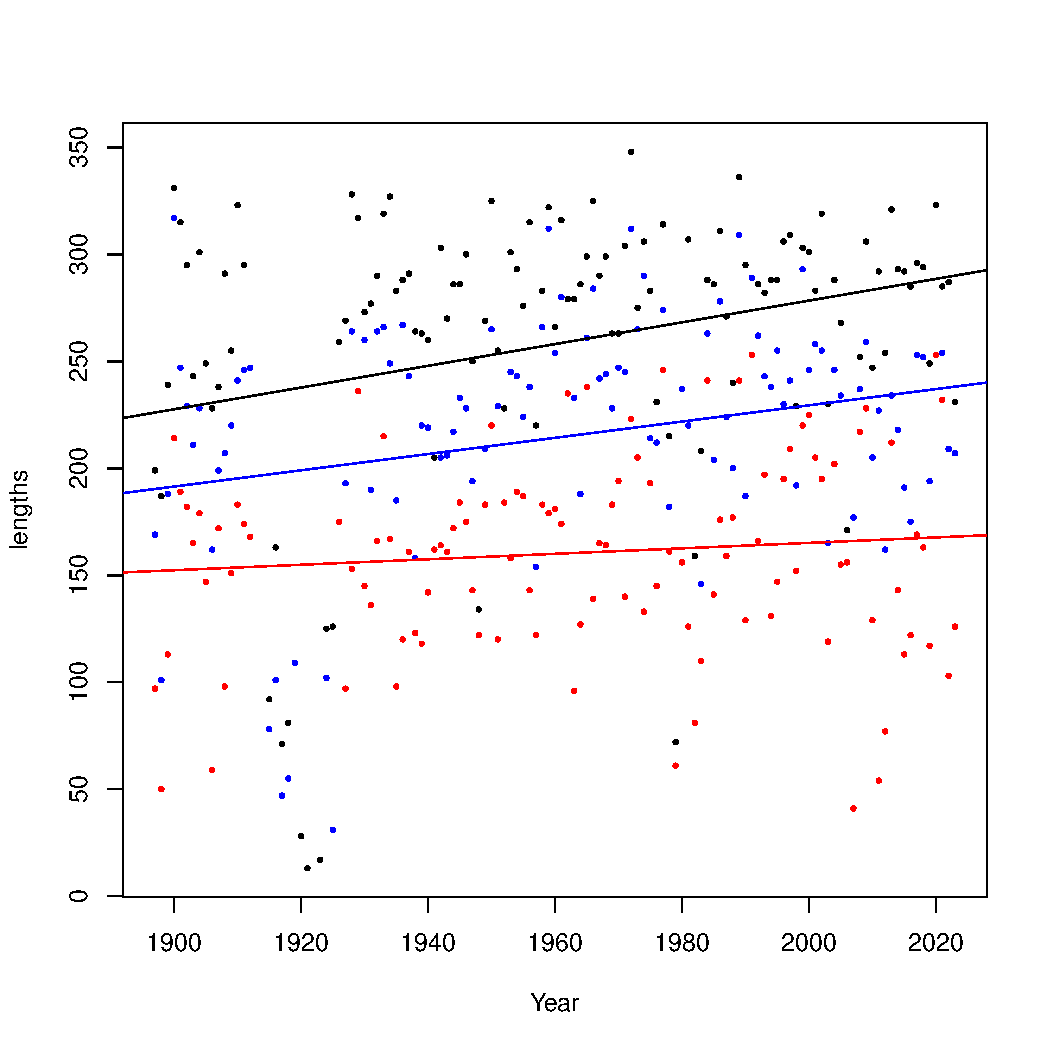
\includegraphics[width=\maxwidth]{figure/unnamed-chunk-10-1} 
\begin{kframe}

{\ttfamily\noindent\bfseries\color{errorcolor}{\#\# Error in is.data.frame(data): object 'Drought.run.100' not found}}

{\ttfamily\noindent\bfseries\color{errorcolor}{\#\# Error in is.data.frame(data): object 'Drought.run.100' not found}}\end{kframe}
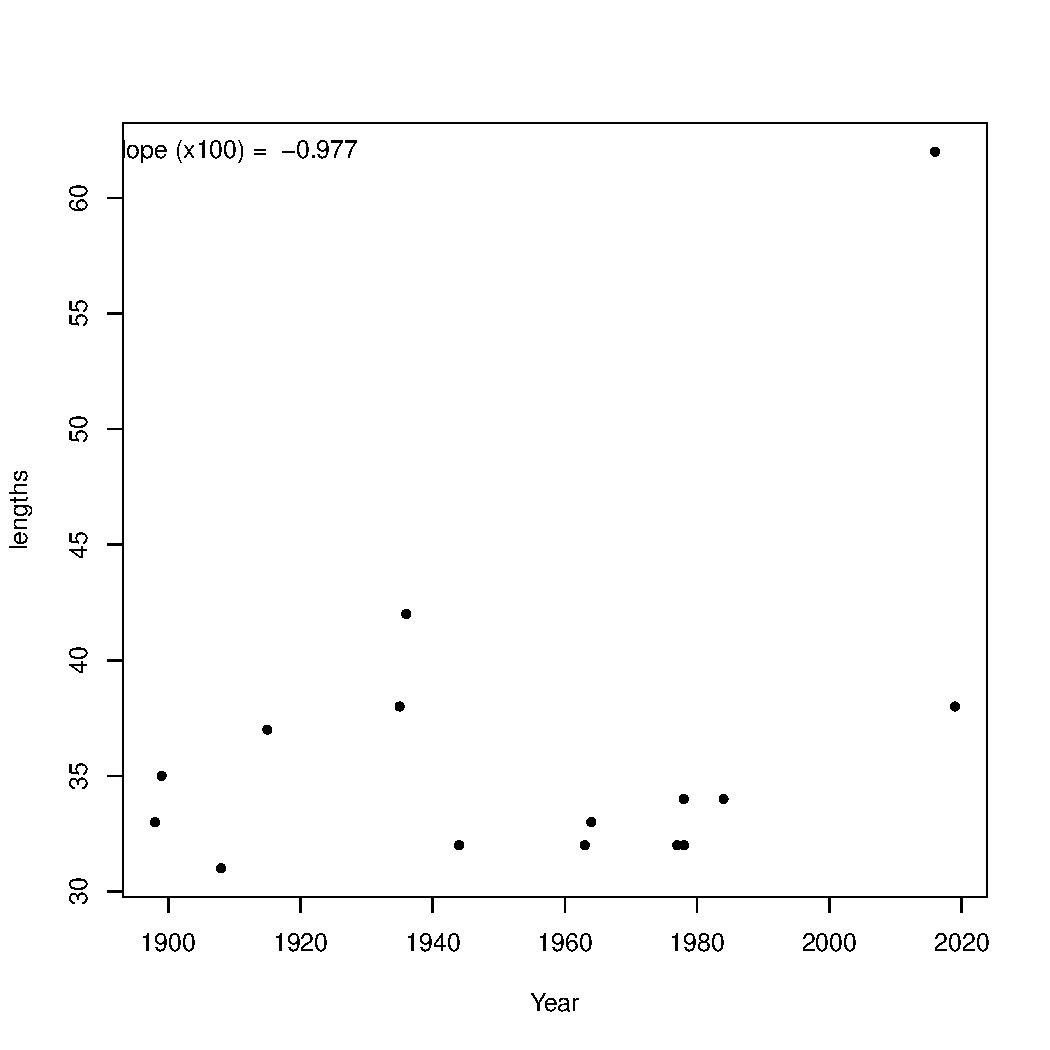
\includegraphics[width=\maxwidth]{figure/unnamed-chunk-10-2} 
\end{knitrout}

Rainfall Probability Distributions by decade... to be developed.





\subsection{Record Setting Temperature Records}

In many cases, people seem to "feel" how temperature has been changing over time, and new records seem to capture the attention in the media. So, we'll create a updated record of maximum temperatures and display them. 





This is a common way to communicate temperatures changes. I suspect we have a better sense of change when we notice "extreme" events...






I tried to use a for loop and in then statements and it was painfully slow, so I converted the data to a matrix that can be used by barplots with much more effeciency!

Create the matrix
\begin{knitrout}
\definecolor{shadecolor}{rgb}{0.969, 0.969, 0.969}\color{fgcolor}\begin{kframe}


{\ttfamily\noindent\bfseries\color{errorcolor}{\#\# Error in TMAX.mat.noleap[j, year.seq\$Col[year.seq\$Year == i]] <- CHCND.noleap\$TMAX[CHCND.noleap\$Year == : replacement has length zero}}\end{kframe}
\end{knitrout}


\begin{knitrout}
\definecolor{shadecolor}{rgb}{0.969, 0.969, 0.969}\color{fgcolor}\begin{kframe}


{\ttfamily\noindent\bfseries\color{errorcolor}{\#\# Error in eval(expr, envir, enclos): no loop for break/next, jumping to top level}}

{\ttfamily\noindent\bfseries\color{errorcolor}{\#\# Error in eval(expr, envir, enclos): no loop for break/next, jumping to top level}}\end{kframe}
\end{knitrout}

The patterns of record temperatures often shows increasing number of new high temperature records  and fewer record low temperatures more recently, but as usual, it depends on the location (Figure~\ref{fig:Records}).
\begin{figure}
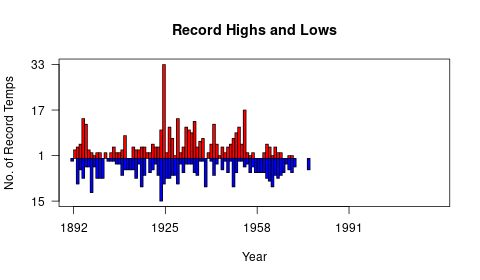
\includegraphics[width=1.00\textwidth]{/home/CAMPUS/mwl04747/github/Climate_Change_Narratives/Social_Media/State_htmls/png/Mississippi_USC00227106_CHCND_Temp_Records.png}
\caption{Daily temperatures that have been the highest on record (in red) and lowest on record (in blue). In some cases, climate change has created more records in the recent decades, while other stations seem don't show that trend.}
\label{fig:Records}
\end{figure}

\subsection{Iterate TMAX vs. Month Boxplots}

Evaluating the changes in TMAX and Monthly temperatures might be useful, but for now, I think it's hard to see the patterns. 




\subsection{Four Plots Compelling Figures}

To test the code, I have created graphics that can then be used in the animation process, i.e. try to create code that doesn't get too complicated and then fail! 

\begin{knitrout}
\definecolor{shadecolor}{rgb}{0.969, 0.969, 0.969}\color{fgcolor}\begin{kframe}


{\ttfamily\noindent\bfseries\color{errorcolor}{\#\# Error in eval(expr, envir, enclos): no loop for break/next, jumping to top level}}

{\ttfamily\noindent\bfseries\color{errorcolor}{\#\# Error in eval(expr, envir, enclos): no loop for break/next, jumping to top level}}\end{kframe}
\end{knitrout}

\begin{figure}
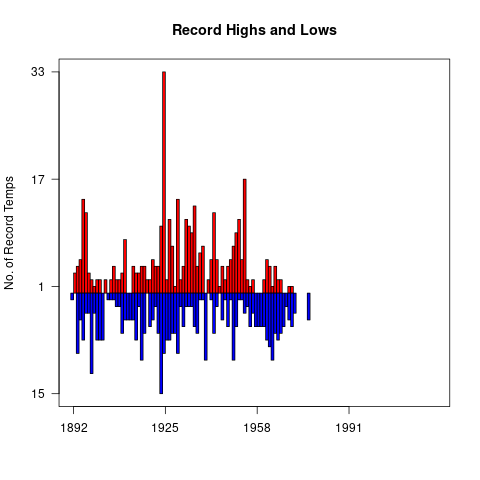
\includegraphics[width=1.00\textwidth]{/home/CAMPUS/mwl04747/github/Climate_Change_Narratives/Social_Media/State_htmls/png/Mississippi_USC00227106_4panel.png}
\caption{Climate can be analyzed using several types of lenses. In this case, we have analyzed show the months with the greatest changes. The first figure is monthly average of TMINs (daily low temperatures) with a best fit line. The second figure shows the monthly TMAX range and asterisks indicate singificant changes over the station record and the third figure is the trend for these TMAXs over time and includes the best fit line. The final figure shows the daily temperatures that have been the highest on record (in red) and the lowest minimum temperatures (in blue). In some cases, climate change has created more records in the recent decades, while other stations seem don't show that trend.}
\label{fig:4panel}
\end{figure}

\subsection{KISS}

Keeping it simple is critical in communicating scientific information. In this section, I try to come up with a consistent message for every state and a simple graphic. 

\subsubsection{Change Point Analysis}
First, TMIN and TMAX and change point analysis...

https://cran.r-project.org/web/packages/mcp/readme/README.html



Let's create a figure that simplifies the narrative, if we can!



\begin{figure}
\includegraphics[width=1.00\textwidth]{/home/CAMPUS/mwl04747/github/Climate_Change_Narratives/Social_Media/State_htmls/png/Mississippi_USC00227106_KISS.png}
\caption{Keep it simple stupid!}
\label{fig:GSOM-KISS}
\end{figure}

\subsection{Temp \& Precipitation Probability}

To highlight the patterns of change, it might be useful to analyze how the probability ditributuion might change -- we can use a normal probability distribion as a theoretical distribution (and we can check if this distribuion is approrpriate with a Chi-Square test), or we can use the data to create a emperical distribution, which is my favored approach. 

I started with decade bins, but used 20 years bins (scores) to simplify the graphics while keeping a pretty good temporal resolution.



This figure is pretty effective, but still needs work. 

\begin{figure}
\includegraphics[width=1.00\textwidth]{/home/CAMPUS/mwl04747/github/Climate_Change_Narratives/Social_Media/State_htmls/png/Mississippi_USC00227106_GSOM_dnorm.png}
\caption{The changing in monthly temperature data, assuming a normal probability distribution.}
\label{fig:GSOM_dnorm}
\end{figure}

\subsection{Using library densEstBayes}

Now, I used a screen split to look at the distribution of the temperate anomolies. First, we look at a simple histogram of the entire dataset. 

\begin{knitrout}
\definecolor{shadecolor}{rgb}{0.969, 0.969, 0.969}\color{fgcolor}
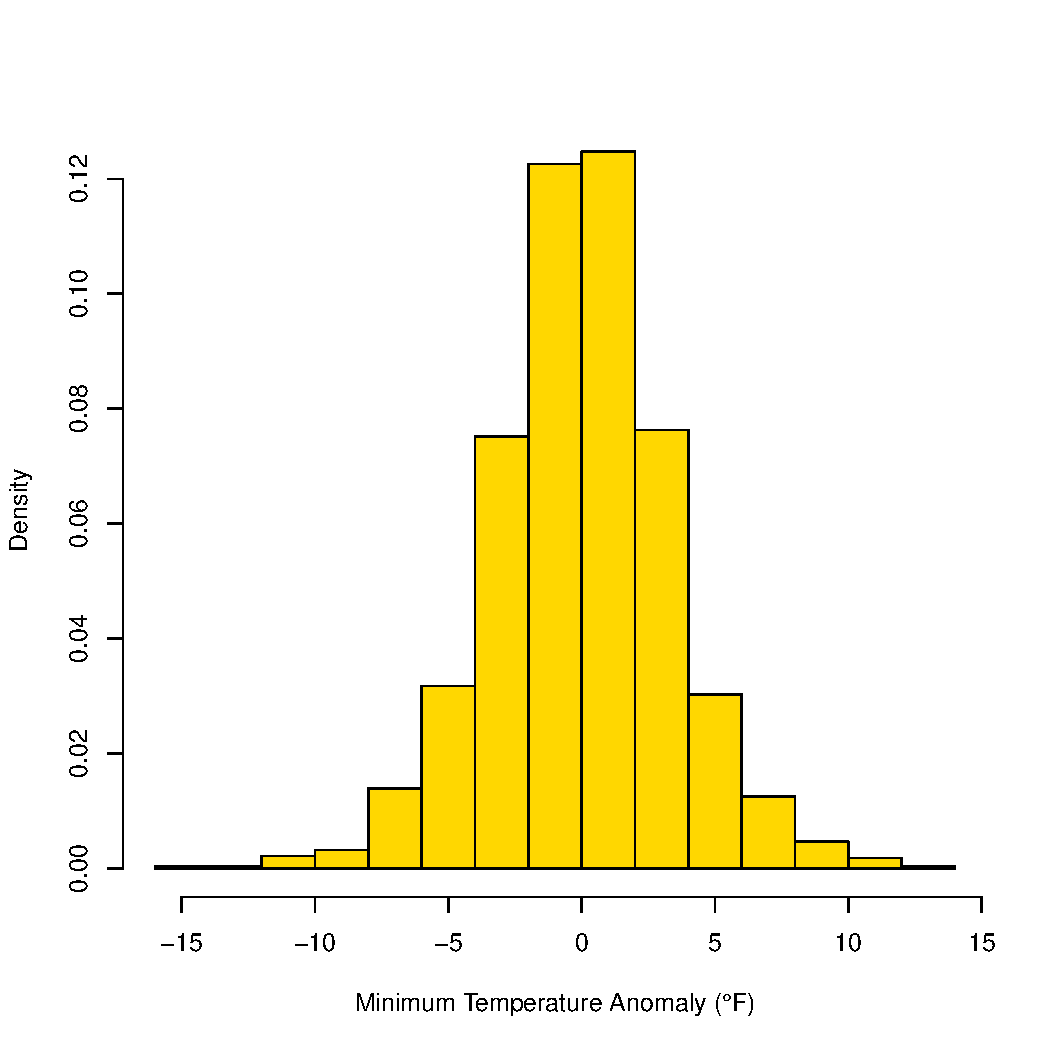
\includegraphics[width=\maxwidth]{figure/unnamed-chunk-16-1} 
\end{knitrout}

The data center around zero, as expected, but are these normally distributed? 

%For TMAX there is a round(shapiro.test(GSOM2$TMAX.anom)$p.value, 7) probability that the distribution is the same as the normal distribution. For TMIN there is a round(shapiro.test(GSOM2$TMIN.anom)$p.value, 7) probability that the distribution is the same as the normal distribution. For PPT is a round(shapiro.test(GSOM2$PPT.anom)$p.value, 7) probability that the distribution is the same as the normal distribution.



These values suggest that there is good reason to avoid  the normal probability distribution. 

Next we use a function to estimate the probability distribution using a markof chain the creates an estimated probability distribution. This doesn't always work when the distribution is not even and their only 10 years of data per slot. I suspect, I should make this by every 20 years. Plus that will go way faster and I think the data visualization will be more robust. 



The process to create these figures is very time consuming, so in general, I need to come up with an if then statement to avoid creating these everytime!

\begin{figure}
\includegraphics[width=1.00\textwidth]{/home/CAMPUS/mwl04747/github/Climate_Change_Narratives/Social_Media/State_htmls/png/Mississippi_USC00227106_GSOM_estPDF.png}
\caption{The changing in monthly temperature data.}
\label{fig:GSOM_estPDF}
\end{figure}

\section{Animated GIFs}

So far, this creates a gif file, but I haven't been able get the gif in the pdf directly yet. I will need an additional package or create separate png that are combined. For now, we'll create a gif file to be used in separate documents.

\subsection{Probability Distributions}




The file is saved in the main directory. 


\subsection{4 Weather Trend Plots}




The file is saved in the main directory. 


\subsection{Evaluating Records}

TBD

\subsection{Export Options}

TBD

\section{Sea Surface Temperature Data -- SURP PROJECT WAITING TO HAPPEN}

In contrast to terrestrial data, sea surface temperature (SST) is quite difficult to obtain and process. There are numerous tools to access the data, but they often require knowledge of complex software tools that are not easy to set up or programming experience with python or others.

\url{https://climexp.knmi.nl/select.cgi?id=someone@somewhere&field=ersstv5}

There are, however, a few tools build for R users that seem to accomplish all that we need. 

\url{https://rda.ucar.edu/index.html?hash=data_user&action=register}

\url{https://rda.ucar.edu/datasets/ds277.9/}

Alternatively, we can download flat ascII tables of gridded data:

\url{https://www1.ncdc.noaa.gov/pub/data/cmb/ersst/v5/ascii/}




\section{Satellite Data}

TBD

\section{Ice-Core Data}

TBD

\section{Conclusions}

Developing a robust method to analyze weather stations is both time consuming and difficult to justify the outcome. In part because the data suggest that each station (region) requires different types of analysis, based on the expected patterns of temperature and rainfall. As climate scientists have known for decades, the terminology of global warming is not very useful. Not because scientists are trying to hide something or promote some biased agenda, but that even as warming of the global average is well documented, the impacts of climate change on each region is highly specific, requiring specificity in the analysis. 

Hopefully, this little analysis has created some mechanism for others to appreciate this compexity. 



The document took 6.3 minutes to process and compile. My next goal will be to optimize the process and streamline the time to analyze. 

\end{document}
